\chapter{Introduction}
\label{cha:intro}
The first section contains a general introduction to the work. The goals are defined and the modus operandi is explained.

\section{Electrocardiograms}
\label{sec:ECG}

% Electrocardiograms (ECGs) are non-invasive recordings that measure the heart's electrical activity using two or more electrodes placed on the skin at the limbs or chest. These electrodes detect the electrical signals that direct the heart muscles to contract, creating a repeating pattern. Various statistics, such as the heart rate, can be readily estimated. However, changes in this electrical pattern can indicate different heart conditions, such as myocardial ischemia, ventricular hypertrophy and conduction problems \cite{m.rangayyanBiomedicalSignalAnalysis2002}.
% \subsection{Background}
% \\ \\
The heart contains a dedicated conduction system that enables electrical signals to travel through it in a coordinated pattern. It consists of specialized elongated muscle cells connected by gap junctions, organized in conducting bundles such as the His bundle and Purkinje fibres, assuring good conductivity through the muscle \cite{villaneloAccessingGapjunctionChannel2017}. Consequently, electrical impulses propagate through numerous fibres simultaneously and can thus be modelled as a surface of current dipoles. Since the human body acts as a volume conductor, this electrical activity can be measured as an electrocardiogram (ECG) between any two electrodes placed on the body, even though the voltage difference is small (at most four mV) \cite{keenerCardiacRhythmicity1998,openstaxCardiovascularSystemHeart2022}.
\\
Specialized regions in the heart, known as nodes, are responsible for controlling this electrical system: these include the sinoatrial (SA) node and the atrioventricular (AV) node. Both nodes function as autonomous oscillators but can be modulated by the endocrine and nervous systems. The SA node serves as the heart's primary pacemaker. When the SA node fires, it generates an action potential (AP) that triggers a precise sequence of excitation and contraction events in the heart muscles. The order of these events is crucial for proper heart function, as illustrated in Figure \ref{fig:heart_conduction}, which shows the different phases of wave propagation through the heart and their correlation with a single-lead ECG \cite{keenerCardiacRhythmicity1998, openstaxCardiovascularSystemHeart2022}.

\begin{enumerate}
    \item The SA node initiates the heartbeat by generating an action potential.
    
    \item This signal spreads through the atria, causing them to depolarize and contract. On the ECG, this is represented as the P wave, which has a small amplitude (0.1–0.2 mV) and lasts about 60–80 ms due to the atria's slow contraction and small size.
    
    \item After the P wave, the signal is delayed at the AV node, creating the PQ segment on the ECG. This is an iso-electric period lasting 60–80 ms.
    
    \item The signal is then rapidly conducted through the His bundle, bundle branches, and Purkinje fibres to the ventricles. Ventricular depolarization begins at the apex and spreads upward, triggering ventricular contraction. This produces the QRS complex on the ECG, a sharp wave lasting approximately 80 ms with an amplitude of about 1 mV. The wave can be either biphasic or triphasic.
    
    \item Following the QRS complex, another iso-electric phase occurs on the ECG spanning about 100–120 ms, called the ST segment. This interval reflects the extended action potential of ventricular cells, which lasts 300–350 ms.
    
    \item Finally, the ventricles repolarize, resulting in the T wave. The T wave has an amplitude of 0.1–0.3 mV and spans 120–160 ms.
\end{enumerate}

\begin{figure}
    \centering
    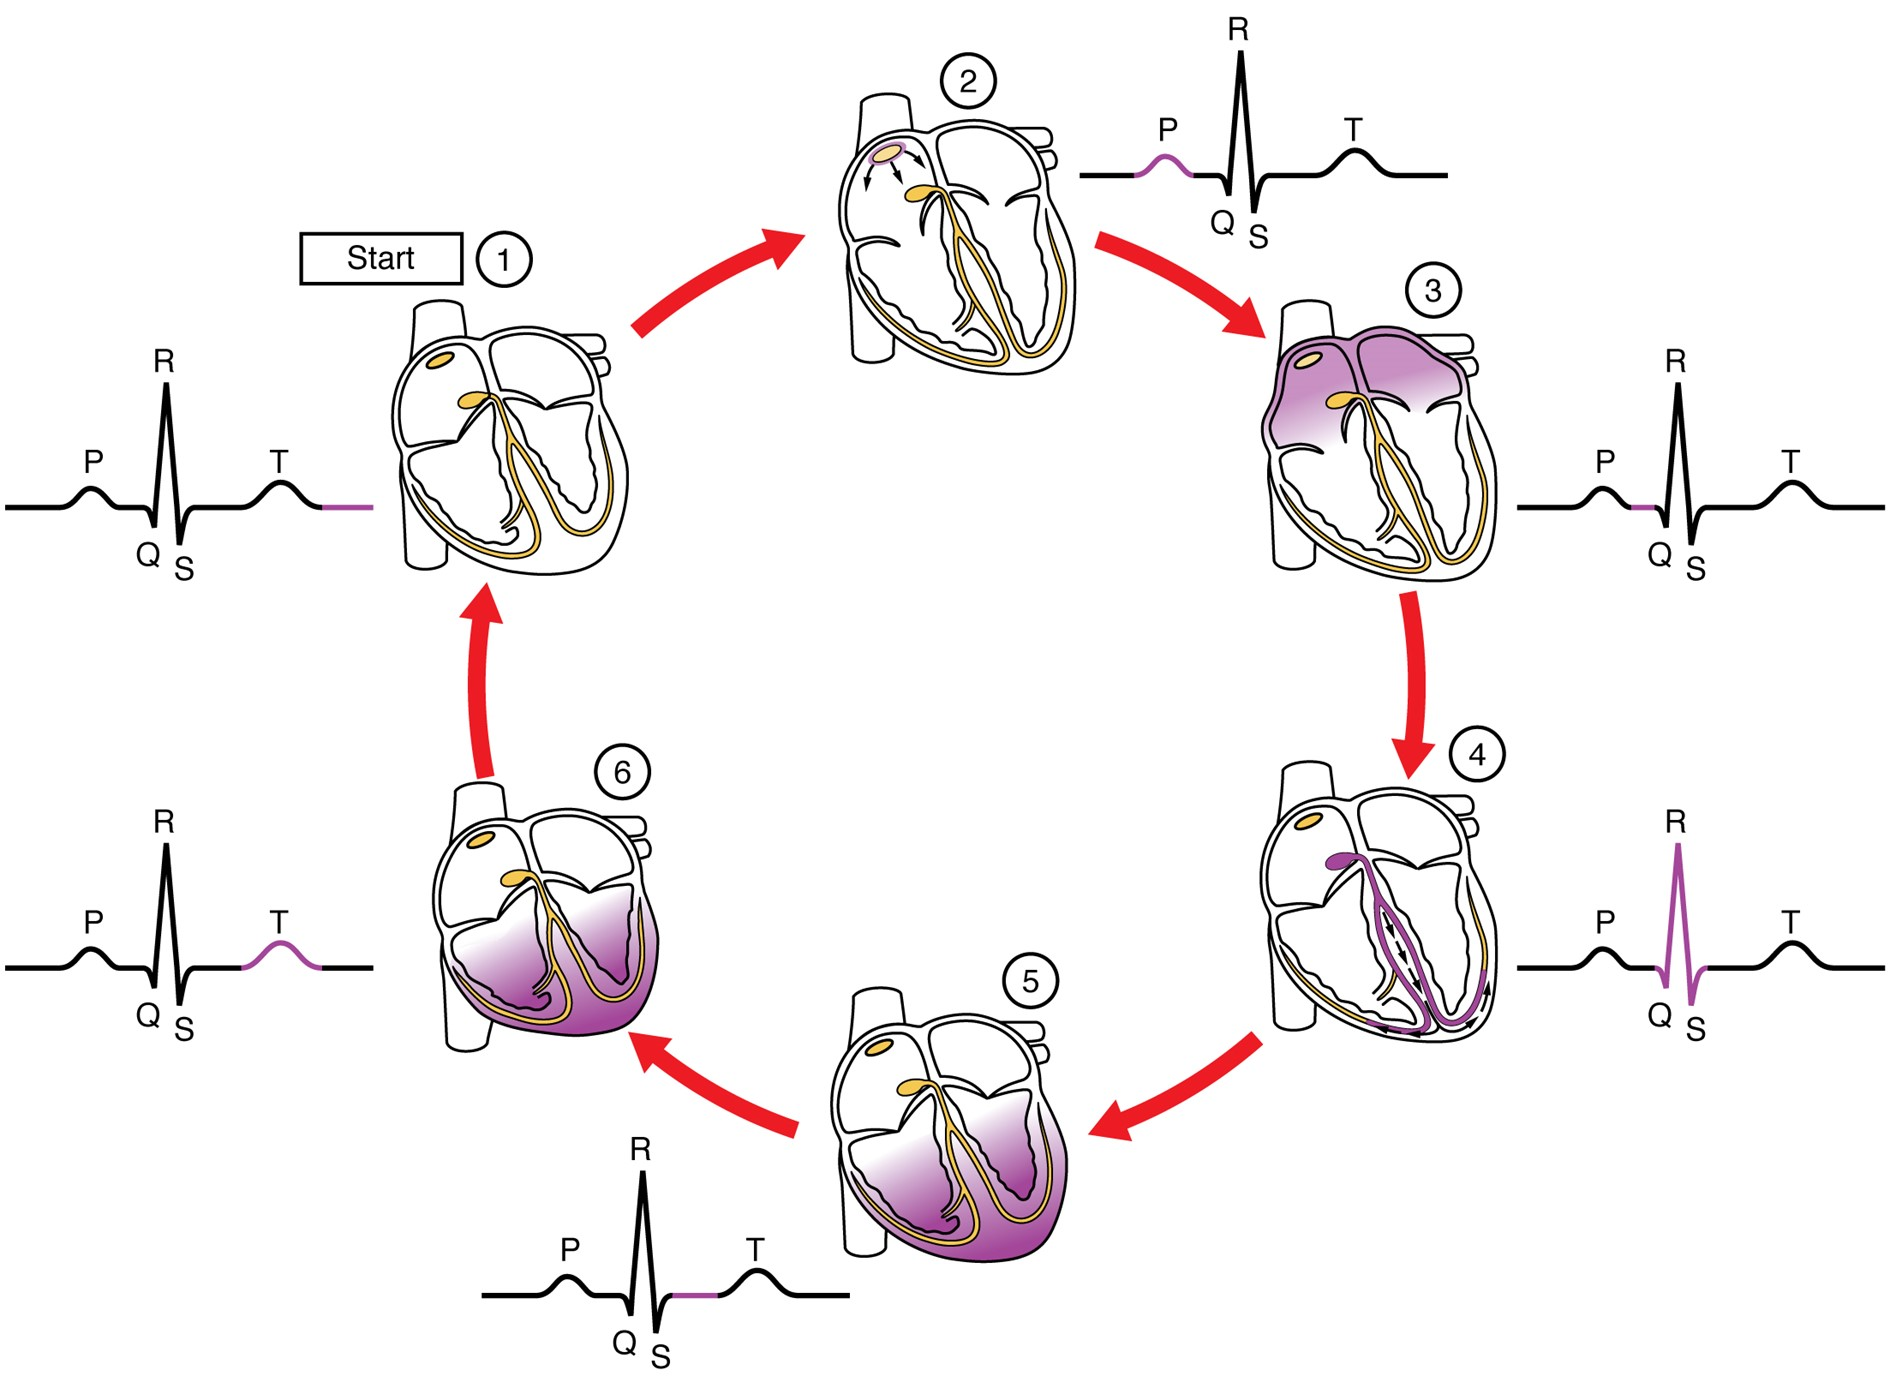
\includegraphics[width=0.7\linewidth]{Figures/1-intro/heart_conduction.jpg}
    \caption{Different phases in the depolarization of the heart correlated with a single-lead ECG (lead II) and its typical waves \cite{openstaxCardiovascularSystemHeart2022}. The SA and AV nodes are indicated in yellow. The purple shading illustrates the propagation of the depolarizing wave through the heart. The purple segments in the ECG lead show which part of the electrical signal corresponds to each phase of cardiac depolarization.}
    \label{fig:heart_conduction}
\end{figure}

\noindent Some events like the repolarization of the atria, the firing of the SA node and Purkinje network propagation are too weak to be detected on the ECG because either not enough heart muscle cells are involved or extracellular current is generated \cite{keenerCardiacRhythmicity1998, m.rangayyanBiomedicalSignalAnalysis2002}. 

\begin{figure}
    \centering
    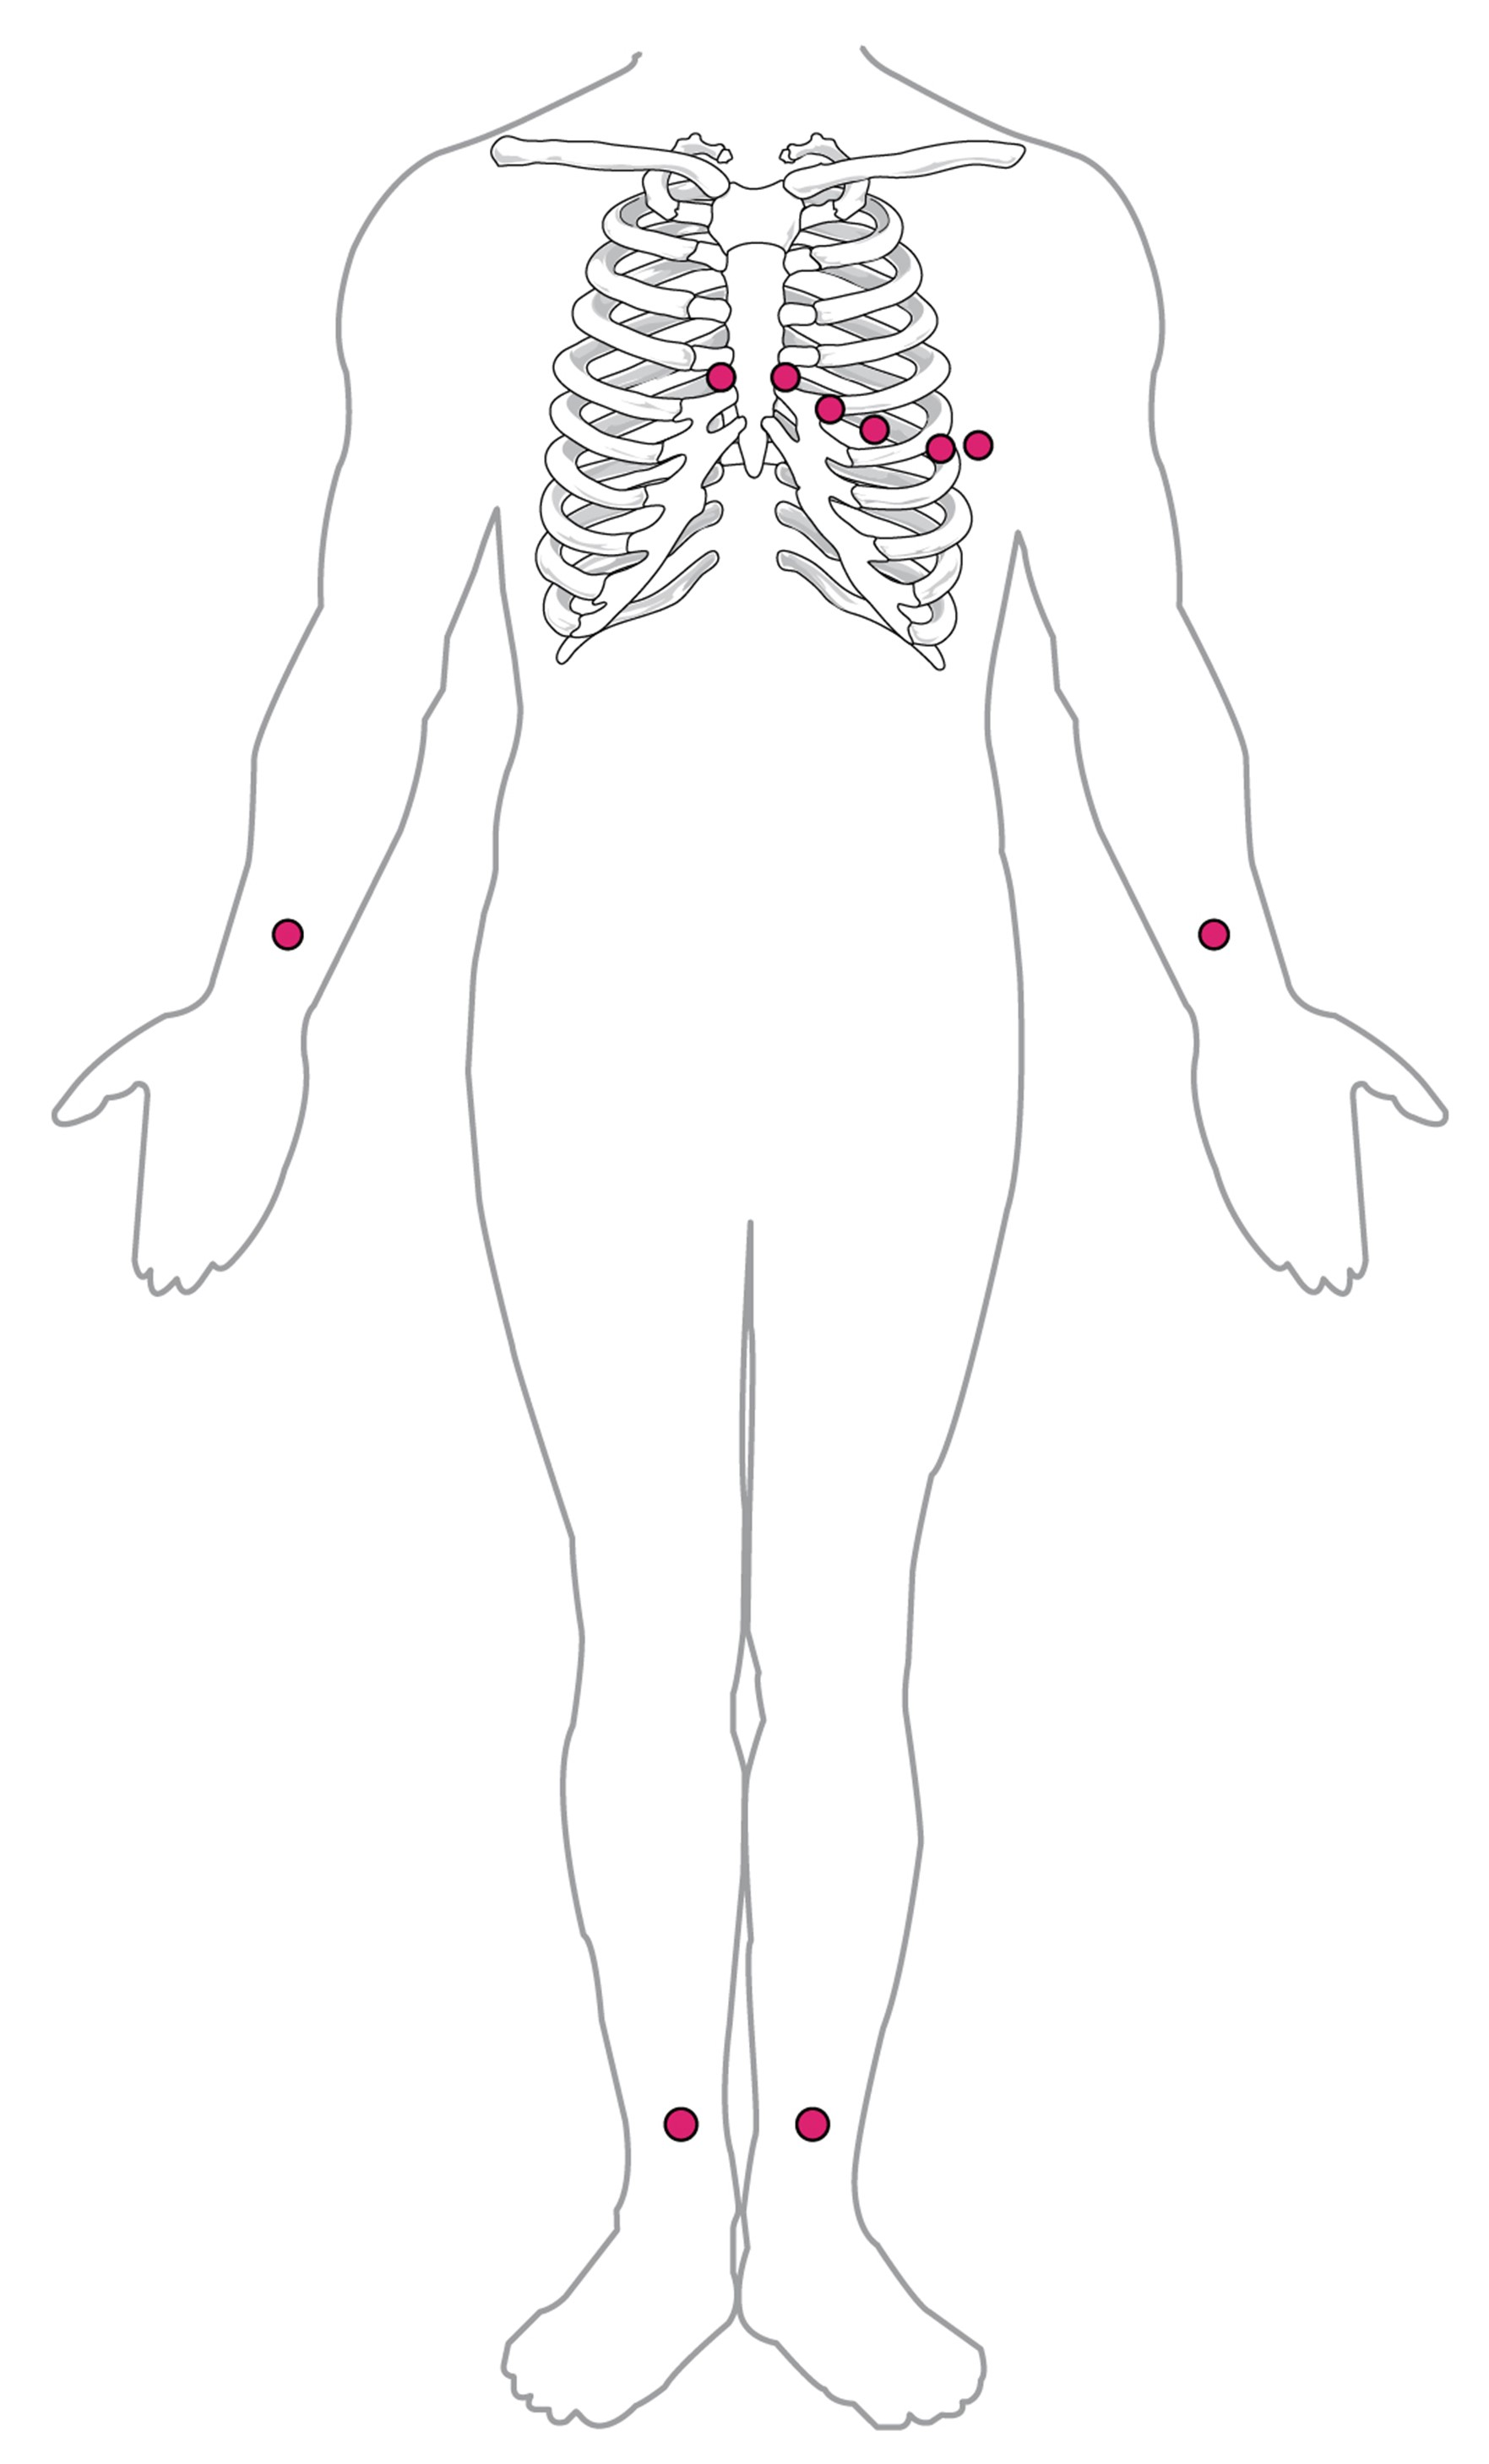
\includegraphics[width=0.25\linewidth]{Figures/1-intro/electrode_placement.jpg}
    \caption{Standard electrode placement for a 12-lead electrocardiogram \cite{openstaxCardiovascularSystemHeart2022}}
    \label{fig:electrode_placement}
\end{figure}

\noindent However, the human body's conductive properties are not homogeneous, as different tissues exhibit varying conductivities, while the presence of aligned fibres in muscles creates anisotropic conditions. To obtain comprehensive information about the heart's electrical activity, clinical practice uses a standardized 12-lead ECG system. This system requires ten electrodes positioned at specific locations on the body with six electrodes placed on the chest and one on each limb, as illustrated in Figure \ref{fig:electrode_placement}, generating twelve different measurement channels called leads \cite{keenerCardiacRhythmicity1998}.

\begin{figure}[h]
    \centering
    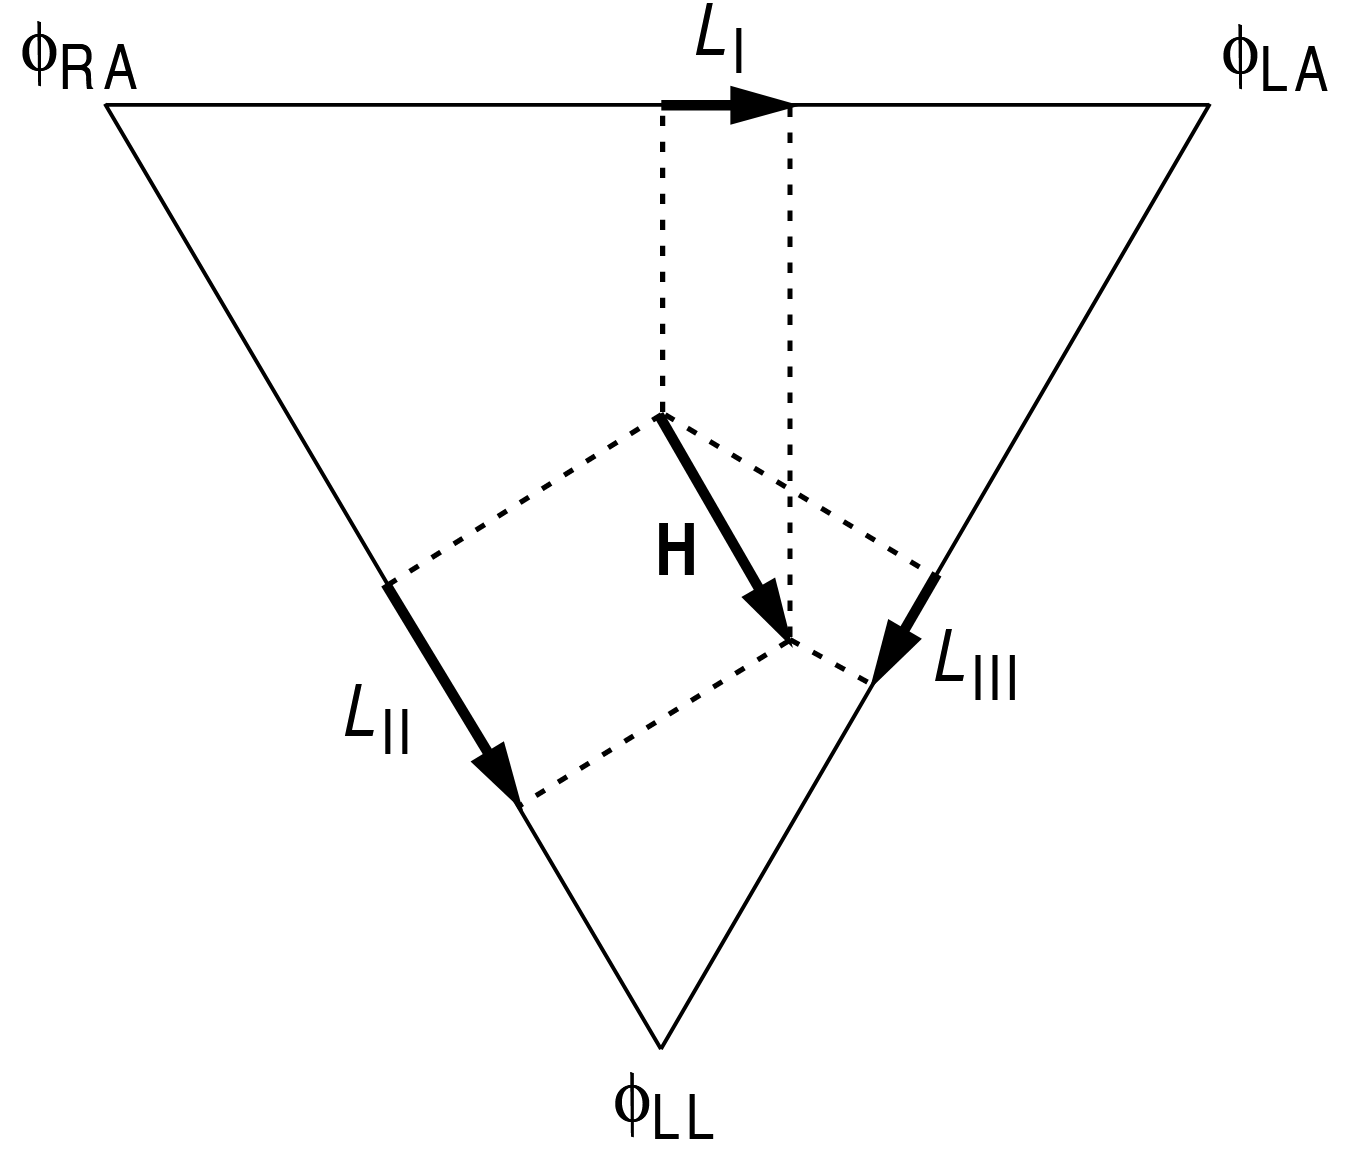
\includegraphics[width=0.35\linewidth]{Figures/1-intro/einthoven_triangle.png}
    \caption{Einthoven's triangle showing a typical heart vector \(\textbf{H}\) and associated lead vectors \cite{keenerCardiacRhythmicity1998}}
    \label{fig:einthoven_triangle}
\end{figure}

\noindent Around the beginning of the twentieth century, Willem Einthoven established the first three leads, which are still used today \cite{rivera-ruizEinthovensStringGalvanometer2008}. By placing electrodes on the left arm (LA), right arm (RA), and left leg (LL), he could measure three different potential differences \cite{keenerCardiacRhythmicity1998}:

\begin{equation}
\begin{split}
I &= \phi_{LA} - \phi_{RA}, \\
II &= \phi_{LL} - \phi_{RA}, \\
III &= \phi_{LL} - \phi_{LA}.
\end{split}
\end{equation}

\noindent This configuration results in two independent equations and one dependent equation \((I + III = II)\) from which information about the frontal plane can be retrieved. These three leads form an equilateral triangle, known as Einthoven's triangle, as illustrated in Figure \ref{fig:einthoven_triangle} \cite{lunaMorphologyElectrocardiogram2005}.
\\ \\
For the 12-lead ECG, three additional leads were introducedin the frontal plane by making linear combinations of the original limb leads. The formulas to derive leads aVR, aVL, and aVF from leads I and II are given by \cite{lunaMorphologyElectrocardiogram2005, zhangSynthesisStandard12lead2021,thambawitaDeepFakeElectrocardiogramsUsing2021}:

\begin{equation}
\begin{bmatrix}
    aVR \\
    aVL \\
    aVF
\end{bmatrix}
=
\begin{bmatrix}
    -\frac{1}{2} & -\frac{1}{2} \\
    +1 & -\frac{1}{2} \\
    -\frac{1}{2} & +1
\end{bmatrix}
\begin{bmatrix}
    I \\
    II
\end{bmatrix}.
\end{equation}

\noindent The six electrodes placed on the chest are used to define the six remaining leads giving information about the horizontal plane. In contrast to the limb leads, Wilson's Central Terminal is defined as a new `zero reference'. This reference is calculated by averaging over leads \(I, II\) and \(III\), and is thus situated in the middle of Einthoven's triangle. The remaining leads are obtained by measuring the potential difference between the chest electrodes and Wilson's Central Terminal.
By analyzing the limb leads and chest leads in conjunction, physicians can track the three-dimensional propagation of electrical signals through the heart. This detailed spatial information, combined with temporal ECG characteristics, allows for the detection of various cardiac abnormalities, making the ECG an essential tool in diagnosing heart conditions and assessing cardiac function \cite{m.rangayyanBiomedicalSignalAnalysis2002}. 
\\ \\
Cardiac electrical activity is monitored in clinical practice through either short-term clinical ECG recordings or long-term Holter monitoring. The standard ten-minute ECG is conducted while patients remain at rest in a controlled clinical setting, providing a focused snapshot of cardiac function. In contrast, Holter monitoring tracks heart activity continuously over 24 hours or more as patients go about their daily routines, offering a more comprehensive view of cardiac behavior across different activities and conditions. While this extended monitoring period reduces patient and staff logistical burden compared to clinical ECG trials and can potentially detect heart conditions which do not appear frequently, recording during regular physical movement makes it more susceptible to movement artifacts and environmental noise that can affect data quality.

% For example, a prolonged QT interval can indicate a risk of sudden cardiac death, while a widened QRS complex can indicate a bundle branch block. The P wave can be used to diagnose atrial fibrillation, while the ST segment can indicate myocardial ischemia \cite{m.rangayyanBiomedicalSignalAnalysis2002}.
% Various statistics, such as the heart rate, can be readily estimated. However, changes in this electrical pattern can indicate different heart conditions, such as myocardial ischemia, ventricular hypertrophy and conduction problems \cite{m.rangayyanBiomedicalSignalAnalysis2002}.

\section{Generative Artificial Intelligence}

Generative models are powerful tools used for tasks such as data augmentation, filling in missing data, protecting privacy, and benchmarking model performance. By creating high-quality synthetic data that closely resembles real data, these models make it possible to expand and diversify datasets in a safe way. This approach is well-established in image data, where it is easy to visually check if the generated samples look realistic. However, there is growing interest in using synthetic data for other types, including time series \cite{mogrenCRNNGANContinuousRecurrent2016, estebanRealvaluedMedicalTime2017, yuSeqGANSequenceGenerative2017, kongDiffWaveVersatileDiffusion2021}, language processing \cite{yuSeqGANSequenceGenerative2017, liAdversarialLearningNeural2017}, and molecular structures \cite{hawkins-hookerGeneratingFunctionalProtein2021, repeckaExpandingFunctionalProtein2021}. In these areas, ensuring authenticity is just as important but can be more difficult to evaluate.
\\ 
A significant challenge in generative modelling is evaluating the synthetic data generated by these models. Various metrics have been proposed for this purpose, each providing different measures of data quality. At the distribution level, maximum mean discrepancy (MMD) assesses how well the underlying data distribution is learned by comparing sample statistics \cite{estebanRealvaluedMedicalTime2017}. For signal-level comparison, several metrics are commonly employed: percentage root mean square difference (PRD) measures the distortion between real and generated signals, while root mean square error (RMSE) evaluates their stability \cite{zhuElectrocardiogramGenerationBidirectional2019}. Signal similarity can be assessed through the Fréchet distance (FD), where a lower value indicates higher quality, and through dynamic time warping (DTW), which has proven particularly effective for time series data \cite{zhuElectrocardiogramGenerationBidirectional2019, delaneySynthesisRealisticECG2019, serraEmpiricalEvaluationSimilarity2014}. Beyond these direct comparison metrics, evaluation can also be performed through classifier-based approaches. The synthetic-to-real (TSTR) method involves training a classifier on synthetic data and testing it on real data to assess whether the generative model produces samples suitable for replacing real data in applications. Conversely, the real-to-synthetic (TRTS) approach evaluates whether the model generates samples with realistic features \cite{estebanRealvaluedMedicalTime2017}.
% \\
% Furthermore the privacy 
% A significant challenge in generative modelling is preventing overfitting to the training data. When a model overfits, it may produce outputs that unintentionally replicate the original data instead of generating new, unique samples. This "data leakage" undermines the privacy benefits of synthetic data, as it can expose sensitive information from the training data \cite{estebanRealvaluedMedicalTime2017}.
\\
The three main types of generative models are variational autoencoders (VAEs) \cite{kingmaAutoEncodingVariationalBayes2013}, generative adversarial networks (GANs) \cite{goodfellowGenerativeAdversarialNetworks2014}, and diffusion models \cite{sohl-dicksteinDeepUnsupervisedLearning2015}. Each has unique strengths: VAEs are good at capturing continuous data distributions, GANs are known for producing high-quality images, and diffusion models are valued for creating stable and diverse samples across many data types \cite{xiaoTacklingGenerativeLearning2022}. The following section provides a detailed overview of these models.

\begin{figure} [h]
    \centering
    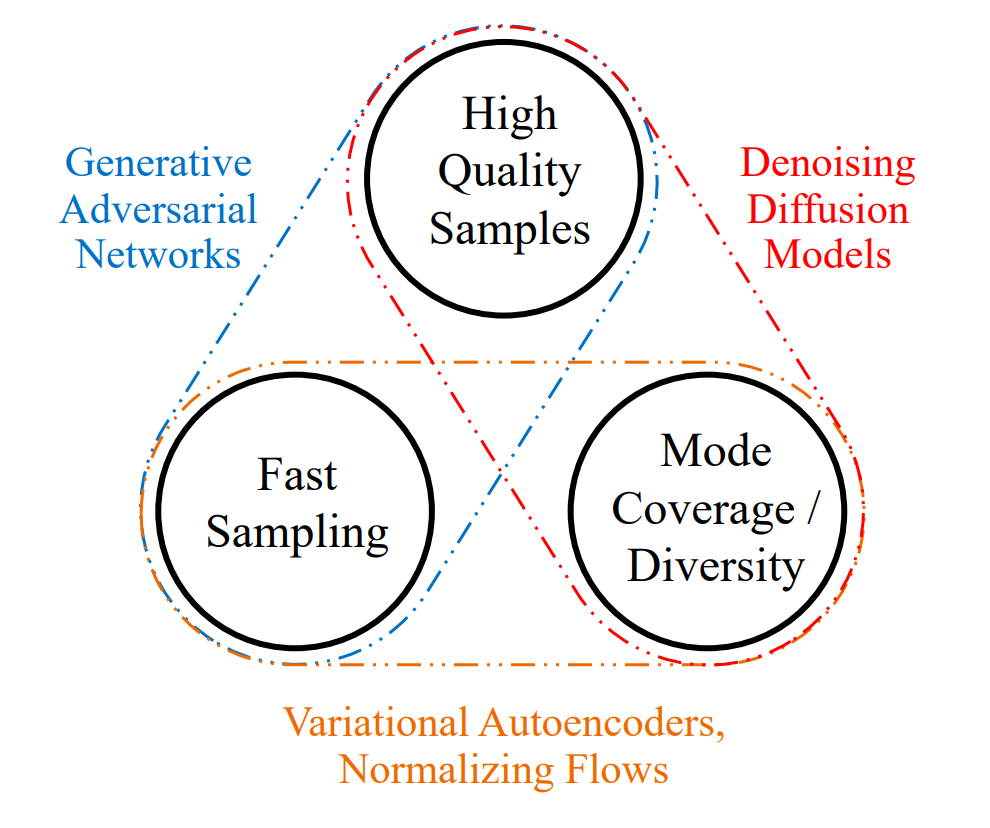
\includegraphics[width=0.35 \linewidth]{Figures/1-intro/GenAI_comparison.png}
    \caption{Comparison between generative artificial intelligence architectures \cite{xiaoTacklingGenerativeLearning2022}}
    \label{fig:GenAI_comparison}
\end{figure}

\subsection{Variational Autoencoders}

Variational Autoencoders (VAEs) are a type of autoencoder that feature a unique structure enabling them to generate new, similar data samples. Like standard autoencoders, VAEs consist of two main parts: an encoder and a decoder. The encoder transforms observed data into latent (hidden) variables, which represent essential information in a compressed form (often referred to as the code). The decoder then takes these latent features and reconstructs them back into the original data space \cite{kingmaAutoEncodingVariationalBayes2013}.
\\
In \cite{kingmaAutoEncodingVariationalBayes2013}, \textit{Kingma et al.} introduced a probabilistic interpretation of autoencoders. VAEs aim to learn the posterior distribution \( p(\mathbf{z}|\mathbf{x}) \), where \( \mathbf{z} \) represents the latent variables and \( \mathbf{x} \) denotes the observed data. However, the true posterior \( p(\mathbf{z}|\mathbf{x}) \) is intractable, so the encoder approximates it with a simpler distribution \( q(\mathbf{z}|\mathbf{x}) \), parameterized by \( \phi \). This approximate distribution is referred to as a recognition model. The decoder then reconstructs data samples by mapping the latent features back to the data space using the likelihood \( p(\mathbf{x}|\mathbf{z}) \), parameterized by \( \theta \) \cite{kingmaAutoEncodingVariationalBayes2013}.
\\
The objective of the VAE is to maximize the marginal likelihood of the observed data \( p(\mathbf{x}) \), but this is intractable to compute directly. Instead, \textit{Kingma et al.} proposed a method to maximize a variational lower bound on this likelihood, known as the evidence lower bound (ELBO) \cite{kingmaIntroductionVariationalAutoencoders2019}:

\begin{equation}
ELBO = \mathbb{E}_{q_\phi(\mathbf{z|x})} \left[ \log p_\theta(\mathbf{x} \mid \mathbf{z}) \right] - \mathrm{KL} \left( q_\phi(\mathbf{z} \mid \mathbf{x}) \, \| \, p_\theta(\mathbf{z}) \right).
\end{equation}

\noindent This bound allows the model to optimize both the \( \theta \) and \( \phi \) parameters jointly, balancing reconstruction accuracy and the divergence between \( q_\phi(\mathbf{z}|\mathbf{x}) \) and the prior distribution \( p_\theta(\mathbf{z}) \). This approach enables VAEs to handle large datasets and approximate complex distributions, making them effective for tasks such as data generation and representation learning \cite{kingmaIntroductionVariationalAutoencoders2019}.

\subsection{Generative Adversarial Networks}

Generative Adversarial Networks (GANs) make use of two networks which try to beat each other in a minimax game. One of the networks, which is called the generator, tries to predict a data sample with noise as input, while the other, the discriminator, tries to differentiate between the real data samples and the generated data samples. This structure is reflected in the objective function \cite{goodfellowGenerativeAdversarialNetworks2014}:

\begin{equation}
V(D, G) = \mathbb{E}_{\mathbf{x} \sim p_{\text{data}}(\mathbf{x})} \left[ \log D(\mathbf{x}) \right] + \mathbb{E}_{\mathbf{z} \sim p_\mathbf{z}(\mathbf{z})} \left[ \log \big( 1 - D(G(\mathbf{z})) \big) \right]
\end{equation}

\noindent which has to be maximized with respect to the discriminator (D) and minimized with respect to the generator (G). 
\\
They have as an advantage high-quality samples and are cheap to sample from. However, a prominent problem of GANs is the variation in the samples which is often called the Helvetica scenario and corresponds to mode collapse. In this scenario, the generator finds a sample that works particularly well against the discriminator and starts only to output this sample \cite{goodfellowGenerativeAdversarialNetworks2014}. 
\\
\textit{Arjovsky et al.} \cite{arjovskyWassersteinGAN2017} propose a solution to this issue, where they substitute the discriminator which normally outputs a probability, with a critic (C) which outputs values on the real axis. Subsequently, the objective function is modified \cite{arjovskyWassersteinGAN2017}:

\begin{equation}
\max_C \min_G \mathbb{E}_{\mathbf{x} \sim p_{\text{data}}(\mathbf{x})} \left[ C(\mathbf{x}) \right] - \mathbb{E}_{\mathbf{z} \sim p_\mathbf{z}(\mathbf{z})} \left[ C(G(\mathbf{z})) \right]
\end{equation}

\noindent which uses the Earth Mover distance, also known as the Wasserstein-1 distance. 
\\
GANs have often been used to generate realistic-looking images as in \cite{radfordUnsupervisedRepresentationLearning2016} where \textit{Radford et al.} propose DCGAN. GANs have also shown promise for generating time series as described in \cite{estebanRealvaluedMedicalTime2017, mogrenCRNNGANContinuousRecurrent2016}.

\subsection{Diffusion Models}

Diffusion models operate through two distinct processes: a forward diffusion process and its corresponding reverse process. During forward diffusion, the data undergoes stepwise degradation through the systematic addition of noise which is often Gaussian. Subsequently, the reverse process aims to reconstruct the original data by progressively removing this noise. This reconstruction is achieved through a neural network that learns to estimate the noise distribution parameters at each step. Specifically, for Gaussian noise the mean \( \mathbf{\mu}_\theta(\mathbf{x}_t, t) \) and variance \( \mathbf{\sigma}^2_\theta \) are estimated at each step, thereby enabling iterative noise removal and data restoration \cite{sohl-dicksteinDeepUnsupervisedLearning2015}. The objective function then becomes maximizing the lower bound on the log-likelihood as in VAEs \cite{hoDenoisingDiffusionProbabilistic2020}:

\begin{equation}
\mathbb{E}_q \left[
    \log p(\mathbf{x}_T) 
    + \sum_{t \geq 1} \log 
    \frac{p_\theta(\mathbf{x}_{t-1} \mid \mathbf{x}_t)}{q(\mathbf{x}_t \mid \mathbf{x}_{t-1})}
\right]
\end{equation}

\noindent \textit{Ho et al.} \cite{hoDenoisingDiffusionProbabilistic2020} changed the objective from learning the mean of the data \( \mu \), to learning the noise \( \epsilon \) instead. The objective function to minimize becomes \cite{hoDenoisingDiffusionProbabilistic2020, kazerouniDiffusionModelsMedical2023}:

\begin{equation}
    \mathbb{E}_{t, \mathbf{x}_0, \mathbf{\epsilon}} \left[
    \left\Vert
    \mathbf{\epsilon} - 
    \mathbf{\epsilon}_\theta \left( \mathbf{x}_t, t \right)
    \right\Vert^2
    \right].
\end{equation}

\noindent Diffusion models generate high-quality samples that are diverse and cover the full data distribution surpassing GANs in image generation \cite{nicholImprovedDenoisingDiffusion2021}. However, due to their iterative nature with small step size, they are computationally expensive to sample \cite{xiaoTacklingGenerativeLearning2022}.
 
\section{Medical Time Series Generation}

The generation of medical time series data using deep learning methods has evolved significantly over recent years. While initial approaches typically focused on generating univariate short segments, more recent methods have demonstrated increasing capability in producing complex multivariate signals. This section examines the key methodological developments in medical time series generation, with particular attention to their applications and limitations.
\\ \\
The application of GANs to medical time series generation was first systematically explored in 2017 by Esteban et al. \cite{estebanRealvaluedMedicalTime2017}. Their approach employs recurrent neural networks (RNNs), specifically long short-term memory networks (LSTMs), for both the generator and discriminator components.
They explored both conditional and non-conditional GAN variants. The generator uses as input a distinct noise sample for each time step of the series, with one conditional parameter in conditional setups. The discriminator assesses the authenticity of each sample point individually and also uses the conditional parameter in conditional setups.
\\
Recognizing the challenges of evaluating medical time series generation, \textit{Esteban et al.} proposed two evaluation frameworks: testing classification models trained on synthetic data against real data (TSTR) and vice versa (TRTS). These approaches provide quantitative metrics for assessing generation quality without relying on costly expert reviews.
To validate these methods, they utilized both synthetic datasets (sine waves and Gaussian processes) and real intensive care unit (ICU) data such as pulse oximeter, heart rate, respiratory rate, and mean arterial pressure signals. These vital measurements were originally recorded every five minutes and then down-sampled by a factor of three. The study focused on sixteen points corresponding to the initial four hours of a patient's stay. 
% I don't see the benefit of using independent latent space samples as the generator's input and classifying each time sample separately by the discriminator. So I will have to test if using only one sample makes a difference.
\\ \\
In a following study, \textit{Zhu et al.} \cite{zhuElectrocardiogramGenerationBidirectional2019} applied a GAN-based architecture to synthetic ECG generation but modified the previous LSTM setup. They replaced the LSTM in the generator with a bidirectional LSTM (BiLSTM), allowing it to consider both past and future values in the time series, and replaced the LSTM in the discriminator with a 1D convolutional network (CNN). CNNs, which are faster to train for long sequences, have shown promise in classification tasks for sequential data such as text and audio \cite{lecunConvolutionalNetworksImages1995}, \cite{kimConvolutionalNeuralNetworks2014}, \cite{zhangCharacterlevelConvolutionalNetworks2016}. 
\textit{Zhu et al.} specifically generated ECG signals between 50 to 400 data points at test-time (0.14s to 1.11s at 360Hz), while their training data consisted of ECGs of 3,120 samples (8.66s at 360Hz). This difference in training-test length is unique and commonly not done. They identified 250 points as optimal based on root mean square error (RMSE) and Fréchet distance (FD) evaluations. Their method, however, was restricted to single-lead ECGs and did not include a conditional framework. The study compared the performance of their GAN architecture with RNN and LSTM models in both autoencoder (AE) and variational autoencoder (VAE) frameworks, noting that the GAN converged more rapidly. Additionally, they tested the 1D-CNN discriminator against multi-layer perceptron (MLP), LSTM, and gated recurrent unit (GRU) based discriminators, finding that the 1D-CNN yielded improved convergence.
\\ \\
In a subsequent comparison, \textit{Delaney et al.} \cite{delaneySynthesisRealisticECG2019} evaluated \cite{estebanRealvaluedMedicalTime2017} and \cite{zhuElectrocardiogramGenerationBidirectional2019} GAN architectures, examining the impact of using a bidirectional LSTM in the generator and a CNN-based discriminator. They tested metrics such as maximum mean discrepancy (MMD) and dynamic time warping (DTW) and conducted preliminary assessments of privacy through a membership inference test.
\\ \\
In another early work, \textit{Golany and Radinsky} \cite{golanyPGANsPersonalizedGenerative2019} devised a method for generating 1-lead personalized ECGs with a GAN. The length of these signals is 216 samples at a sampling rate of 360 Hz. They tried to match the wave features (P, Q, R, S, T) by heuristically adding an MSE loss to the generator objective function. By first training a general GAN network and then further training on personalized data, they were able to obtain more patient-specific samples. They evaluated their approach by training a classifier and comparing the average Area Under Curve (AUC) to different approaches. 
\\ \\ 
In \cite{brophyQuickEasyTime2019}, \textit{Brophy et al.} take a different approach, generating 1-lead ECGs based on images via GANs. They transform the time series into an image format by using the amplitude as a grayscale value and ordering the data into a rectangular format. Because of using this image-based format, they can use proven concepts from GAN image generation, improving training stability. This enables them to generate sequences of 4096 data points at 5 kHZ.
\\ \\
In 2020, \textit{Brophy} \cite{brophySynthesisDependentMultichannel2020} was the first to extend the generation of ECGs to a multivariate 2-lead setup. He uses a GAN with an LSTM network in the generator and a 2D CNN as the discriminator. The signals generated are of length 187. He uses MMD and DTW to evaluate these signals, where DTW is generalized to a multivariate setting. To assess privacy risks he performs a membership inference attack.
\\ \\
\textit{Kuznetsov et al.} \cite{kuznetsovElectrocardiogramGenerationFeature2020} focus mainly on automatically an interpretable set of features encoded in the latent space of their VAE architecture. They note that these features can be further used in automatic diagnostic systems. This approach enables them to generate ECGs with 400 data points at a sample rate of 500 HZ. The encoder and decoder networks both use CNNs in parallel with MLPs where the outputs are concatenated and then put into other MLPs. To evaluate their approach they use MMD. They also evaluated the interpretability of their feature space by each time varying one of the features and looking at the generated samples.
\\ \\
\textit{Golany et al.} propose in \cite{golanySimGANsSimulatorBasedGenerative2020} a framework based on their previous work \cite{golanyPGANsPersonalizedGenerative2019} and on \cite{shrivastavaLearningSimulatedUnsupervised2017} applied in the image domain, using an ECG simulator in the loss function of the generator of a GAN to synthesize ECGs with realistic morphology and characteristics. Similarly to \cite{golanyPGANsPersonalizedGenerative2019}, they use an additional MSE loss, but this time they use the simulator simulated samples to calculate it on. They call this modified loss the Euler loss. They still produce ECGs of 216 samples at 360 Hz. However, in this work, they use instead of their MLP in the generator and 1D CNN in the discriminator, 1D CNNs in both the generator and discriminator. For their evaluation they employ the same method as before, using a classifier and comparing Precision-Recall curves between relevant settings. Like this they show using the simulated samples as input like in \cite{shrivastavaLearningSimulatedUnsupervised2017}, performs worse than including them in the loss function. They also compare their output visually with real examples.
\\ \\
\textit{Wulan et al.} \cite{wulanGeneratingElectrocardiogramSignals2020} designed three different models to generate synthetic ECG signals, which they claim are more realistic and can last up to 20 seconds. The first model is inspired by WaveNet \cite{oordWaveNetGenerativeModel2016}, an autoregressive model initially developed for audio generation, chosen due to its suitability for producing long, sequential signals. However, the sequential nature of this model results in slower training and generation compared to parallel methods, such as GANs. To address this limitation, \textit{Wulan et al.} also proposed two GAN-based models that offer faster generation times based on \cite{radfordUnsupervisedRepresentationLearning2016} and \cite{gulrajaniImprovedTrainingWasserstein2017}. Both approaches use a transformation to another domain. One uses the short-time-Fourier transform (STFT) to get a 2D time-frequency representation of the signal. They call this model SpectroGAN. The other uses the Wavelet Transform (WT) to get a multiresolution analysis of the signal. They call this model WaveletGAN. Contrary to most of the previous works, they propose a conditional framework where they include three different conditions. They train their architectures sequentially on harder tasks through the design of datasets of each time higher complexity. To validate their models they use TSTR and TRTS. With these metrics, they concluded that WaveletGAN performed best out of the three models in terms of producing high-quality data and matching the data distribution. However, their model based on WaveNet can produce time series of arbitrary length.
\\ \\
\textit{Dasgupta et al.} \cite{dasguptaCardioGANAttentionbasedGenerative2021} pointed out that previous synthetic ECGs did not effectively capture physiological patterns found in real ECGs, such as the P wave, QRS complex, and T wave. They introduced an attention mechanism in the generator, alongside a bidirectional LSTM, to better learn the dependencies among these patterns. This adjustment enabled the generation of longer sequences (512 time steps, equivalent to 2.84s at 180Hz). To address training instability, they replaced the traditional GAN loss \cite{goodfellowGenerativeAdversarialNetworks2014} with the Wasserstein loss introduced by \textit{Arjovsky et al.} \cite{arjovskyWassersteinGAN2017}, where the discriminator produces a real-valued “score” rather than a probability. This approach stabilized training, particularly when using complex models in the generator, like attention blocks. However, like previous models, their approach only generated single-lead ECGs and did not incorporate a conditional framework.
They compared their model to state-of-the-art approaches \cite{zhuElectrocardiogramGenerationBidirectional2019} as well as other generative frameworks (AE, VAE) and a traditional non-deep learning method \cite{mcsharryDynamicalModelGenerating2003}. Four evaluation metrics were used: Percentage Root Mean Square Difference (PRD), RMSE, FD, and DTW.
\\ \\
The first study to generate 12-lead ECGs was conducted by \textit{Zhang and Babaeizadeh} \cite{zhangSynthesisStandard12lead2021}. They built on a prior model by \textit{Zhu et al.} \cite{zhuElectrocardiogramGenerationBidirectional2019}, modifying the generator architecture by replacing the 1D BiLSTM with a 2D version. The second dimension was used to capture the physiological and spatial correlations between the leads of the same recording. In the discriminator, they similarly used a 2D CNN instead of the original 1D version. They generated 8 out of the 12 leads and then completed the set by applying rules detailed in Section \ref{sec:ECG}. For labelling consistency, they used the Philips DXL ECG algorithm, assigning one of four labels to each ECG: left ventricular hypertrophy (LVH), left bundle branch block (LBBB), acute myocardial infarction (ACUTMI), and Normal. 
In their approach, they used an unconditional setting, splitting their database by class and training a separate GAN for each label. Each signal was a time series of 800 ms centred around the QRS complex, sampled at 500 Hz. 
\\
To generate ECG signals, they used a unique technique, generating ECGs during training and applying plausibility criteria to ensure quality. The criteria required: (1) the MMD between generated and test ECGs to be less than 0.004, (2) an amplitude range exceeding 1.2 mV, (3) the signal's maximum not falling in the first or last 50 samples, and (4) at least 10 training epochs. For generating multiple ECGs, they proposed continuing training based on prior epochs for each new ECG. To produce a 10-second ECG, they concatenated the same generated segment, enabling the DXL algorithm to validate class labels and calculate a success rate.
\\
To evaluate the synthetic data, they compared the statistical features of the generated ECGs to those of the training set. They also computed PRD and RMSE between the synthetic signals and both the training and test datasets, as well as between the test and training datasets.
\\ \\
\textit{Thambawita et al.} \cite{thambawitaDeepFakeElectrocardiogramsUsing2021} were the first to generate extended ECG signals of up to 10 seconds in length for a 12-lead setup. They introduced a modified version of WaveGAN, called WaveGAN*, as well as a custom network featuring a 1D U-Net-based generator named Pulse2Pulse to produce 8 ECG channels, which could be expanded to 12 leads using standard formulas, as described in Section \ref{sec:ECG}. To maintain consistency, only ECGs classified as normal by the MUSE 12SL (GE Healthcare) system were used for training, thereby avoiding a mix of healthy and pathological ECGs. They validated the quality of generated ECGs by examining heart rate, P wave, QRS complex, T wave, and underlying dependencies through statistical comparisons. Their findings showed that the Pulse2Pulse model outperformed WaveGAN* in both training efficiency and performance, as assessed by the fraction of ECGs classified as normal by MUSE. Similar to previous studies, no conditional framework was employed.
\\ \\
\textit{Brophy et al.} \cite{brophyMultivariateGenerativeAdversarial2021} build further on their previous work \cite{brophySynthesisDependentMultichannel2020}. In this study, they explore different loss functions for the GAN architecture while also increasing the number of data points to 500 at a sample rate of 100 Hz. They keep their model architecture the same. The model is implemented without conditional parameters. By introducing the DTW in the loss function of the discriminatory, they want to improve the stability while training. By using the same metrics as before they show that good results can be achieved without stability issues. They also compare their proposed model to an LSTM network and VAE for generating ECGs. 
\\ \\
In \cite{sangGeneration12LeadElectrocardiogram2022}, \textit{Sang et al.} propose a conditional variational autoencoder (VAE) to generate 12-lead ECG signals that can be tailored to specific subject characteristics, such as age, sex, BMI, heart position, and orientation. They chose the VAE architecture due to its more interpretable latent space compared to GANs. The architecture they employed was inspired by the work of \textit{Ozan et al.}, who developed a similar model for generating EEG signals. In addition to the conditional VAE, they also implemented an unconditional VAE model. To evaluate the performance of the unconditional VAE, they utilized MMD, comparing it between 1,000 randomly sampled real ECG signals and generated ECGs and also against the MMD results obtained in a prior study by \textit{Kuznetsov et al.} \cite{kuznetsovElectrocardiogramGenerationFeature2020}. The conditional VAE was used to explore the relationships between latent space variables, conditional labels, and generated results. This evaluation involved visualizing different leads for inspection and comparing them with clinical data.
\\ \\
To this point, no diffusion model-based architectures had been proposed. In 2023, \textit{Alcaraz and Strodthoff} introduced a diffusion-based approach to generate 10-second, 12-lead ECGs \cite{alcarazDiffusionbasedConditionalECG2023}. Their architecture builds on DiffWave \cite{kongDiffWaveVersatileDiffusion2021}, replacing its dilated convolutional layers with Structured State Space Sequence Model (SSSM) blocks, known as S4 layers. For comparison with relevant state-of-the-art methods, they implemented conditional versions of both WaveGAN* and Pulse2Pulse from \textit{Thambawita et al.} \cite{thambawitaDeepFakeElectrocardiogramsUsing2021}, although the original source code for these networks was unavailable. \textit{Alcaraz and Strodthoff} also attempted to adapt other existing models \cite{yoonTimeseriesGenerativeAdversarial2019, liTTSGANTransformerbasedTimeSeries2022, sangGeneration12LeadElectrocardiogram2022} to generate ECGs with 1000 samples at a rate of 100 Hz, but these models could not achieve the required length, even when downscaled to 250 time steps. For evaluation, they trained a classifier for TSTR and TRTS comparisons and performed a clinical Turing test to assess the realism of the synthetic data. Unlike most prior models, their approach utilized a conditional framework. Similar to \textit{Sang et al.} \cite{sangGeneration12LeadElectrocardiogram2022}, they explored the relationships in modifying the conditional input to the generated signals. Finally, they concluded their model improves on \cite{thambawitaDeepFakeElectrocardiogramsUsing2021}, but still could not compensate for real samples.
\\ \\
Concurrently \textit{Adib et al.} \cite{adibSyntheticECGSignal2022} designed a model based on the improved DDPM \cite{nicholImprovedDenoisingDiffusion2021}. To keep the architecture the same as in \cite{nicholImprovedDenoisingDiffusion2021} they transform a 1-lead time-series into a 3-channel image. They compare this model across different hyperparameters and to a GAN-based model applied to the original 1D signal. With their approach they generate 256 data points at 4 Hz. To evaluate the models they use DTW, FD, MMD and a classification task to test authenticity where they look at the average precision and the AUC for the Precision-Recall Curve (PRC) and Receiver Operator Curve (ROC). From these tests, they concluded the GAN model performed better than the DDPM proposing the DDPM should be applied ideally to 1D data instead of artificial 2D data to make a fair comparison.
\\ \\ 
Following up on \textit{Alcaraz and Strodthoff} \cite{alcarazDiffusionbasedConditionalECG2023}, \textit{Zama and Schwenker} introduced the DSAT-ECG model, a diffusion-based approach to generate 10-second, 12-lead ECGs using a State Space Augmented Transformer (SPADE) architecture \cite{zamaECGSynthesisDiffusionBased2023}. Their model replaces the S4 layers with SPADE to handle the complex dependencies in ECG data.
For comparison, \textit{Zama and Schwenker} evaluated their model against baseline methods including SSSD-ECG \cite{alcarazDiffusionbasedConditionalECG2023}, WaveGAN*, and Pulse2Pulse \cite{sangGeneration12LeadElectrocardiogram2022}. For quality evaluation, they used DTW and MMD and also performed an authenticity assessment like in \cite{alcarazDiffusionbasedConditionalECG2023}. \textit{Zama and Schwenker} concluded that DSAT-ECG outperformed prior models like SSSD-ECG. Although DSAT-ECG does not fully replace real samples for classifier training, it has high fidelity, bringing ECG synthesis closer to clinical application standards. Future directions include exploring trainable variances and latent diffusion for improved speed and quality.
\\ \\


\begin{table}[ht]
\centering
\caption{Comparison of Approaches for Synthetic ECG Generation}
\label{tab:ECG_comparison}
\small
\begin{tabular}{|p{1.5cm}|p{2.3cm}|p{1.8cm}|p{1cm}|p{1.8cm}|p{1cm}|p{1.8cm}|p{0.7cm}|}
\hline
\textbf{Study} & \textbf{Archit.} & \textbf{Dataset} & \textbf{Cond.} & \textbf{Length (sample rate)} & \textbf{Leads} & \textbf{Metrics} & \textbf{Year} \\
\hline
Esteban et al. \cite{estebanRealvaluedMedicalTime2017} & LSTM (G \& D) & Philips eICU & Yes & 16 (1/15min) & 1 & MMD, TSTR, TRTS & 2017 \\
\hline
Zhu et al. \cite{zhuElectrocardiogramGenerationBidirectional2019} & BiLSTM (G) 1D CNN (D) & 3120-sample ECG & No & 50-400 (360Hz) & 1 & PRD, RMSE, FD & 2019 \\
\hline
Golany \& Radinsky \cite{golanyPGANsPersonalizedGenerative2019} & MLP (G) 1D CNN (D) & MIT-BIH & No & 216 (360Hz) & 1 & Classification & 2019 \\
\hline
Delaney et al. \cite{delaneySynthesisRealisticECG2019} & BiLSTM (G) CNN (D) & Eval. of Esteban (2017), Zhu (2019) & No & - & 1 & MMD, DTW, membership inference & 2019 \\
\hline
Brophy \cite{brophySynthesisDependentMultichannel2020} & LSTM (G) 2D CNN (D) & MIT-BIH & No & 187 (/) & 2 & MMD, DTW, membership inference & 2020 \\
\hline
Kuznetsov et al. \cite{kuznetsovElectrocardiogramGenerationFeature2020} & CNN \& MLP (Enc \& Dec) & LU Cardiography & No & 400 (500Hz) & 1 & MMD & 2020 \\
\hline
Golany et al. \cite{golanySimGANsSimulatorBasedGenerative2020} & 1D CNN (G \& D) & MIT-BIH & No & 216 (360Hz) & 1 & Classification & 2020 \\
\hline
Wulan et al. \cite{wulanGeneratingElectrocardiogramSignals2020} & WaveNet \cite{oordWaveNetGenerativeModel2016}, DCGAN \cite{radfordUnsupervisedRepresentationLearning2016} & MIT-BIH & Yes & 1440 (360Hz) 250 (360Hz) & 1 & TSTR, TRTS & 2020 \\
\hline
Dasgupta et al. \cite{dasguptaCardioGANAttentionbasedGenerative2021} & BiLSTM + Attn. (G) (D) & ECG (P, QRS, T) & No & 512 (2.84s) & 1 & PRD, RMSE, FD, DTW & 2021 \\
\hline
Zhang et al. \cite{zhangSynthesisStandard12lead2021} & 2D BiLSTM (G) 2D CNN (D) & PTB-XL, CCDD, CSE, Chapman and private & No & 400 (500Hz) & 12 & PRD, RMSE & 2021 \\
\hline
Thambawita et al. \cite{thambawitaDeepFakeElectrocardiogramsUsing2021} & U-Net (G) CNN (D) & 10s, 12-lead ECG, normal only & No & 10s & 12 & - & 2021 \\
\hline
Brophy et al. \cite{brophyMultivariateGenerativeAdversarial2021} & 2D LSTM (G) 2D CNN (D) & MIT-BIH & No & 500 (100Hz) & 2 & MMD, DTW, membership inference & 2021 \\
\hline
Sang et al. \cite{sangGeneration12LeadElectrocardiogram2022} & 2D CNN (Enc) 2D CNN (Dec) & UK Biobank & Yes & 400 (500Hz) & 12 & MMD & 2022 \\
\hline
Alcaraz \& Strodthoff \cite{alcarazDiffusionbasedConditionalECG2023} & DDPM \cite{nicholImprovedDenoisingDiffusion2021} & PTB-XL & Yes & 1000 (100Hz) & 12 & TSTR, TRTS, Turing & 2023 \\
\hline
Adib et al. \cite{adibSyntheticECGSignal2022} & DDPM \cite{nicholImprovedDenoisingDiffusion2021} & MIT-BIH & No & 256 (64Hz) & 1 & MMD, FD, DTW, Classification & 2023 \\
\hline
Zama \& Schwenker \cite{zama_ecg_2023} & DDPM \cite{nicholImprovedDenoisingDiffusion2021} & PTB-XL & Yes & 1000 (100Hz) & 12 & TSTR, TRTS, Turing & 2023 \\
\hline
\end{tabular}
\end{table}




%%% Local Variables: 
%%% mode: latex
%%% TeX-master: "thesis"
%%% End: 
